
\chapter{Resultados del experimento y detecci\'on de ansiedad}\label{capit:cap4}
\vspace{-2.0325ex}%
\noindent
\rule{\textwidth}{0.5pt}
\vspace{-5.5ex}% 
\newcommand{\pushline}{\Indp}% Indent puede ir o no :p

\section{Introducci\'on}\label{cap4:intro}
En este cap\'itulo se presentan el conjunto de se\~nales fisiol\'ogicas obtenidas del experiment descrito en el cap\'itulo anterior y las caracater\'isticas que se calcularon a partir de estas se\~nales. Se muestran observaciones hechas sobre los datos de manera general y de casos espec\'ificos \'utiles a considerar en la detecci\'on de ansiedad. Por \'ultimo se muestran los resultados de las diferentes pruebas de clasificac\'ion hechas sobre el conjunto de datos.

\section{Resultados generales}
Todas las sesiones se llevaron a cabo del 8 de Julio hasta el 30 de Julio del 2015. Se recolectaron datos de 29 sesiones de las 30 planeadas para el experimento. La sesi\'on faltante pertence a un participante que cancel\'o su tercera participaci\'on debido a problemas de agenda. Por cada sesi\'on se tomaron datos de tres dispositivos. Cada dispositivo captur\'o diferentes se\~nales del usuario. La lista completa de los datos se encuentra en la tabla ~\ref{table:signalsperdevice}.

%inserta tabla aqui%
        \begin{table}[h!]
                \footnotesize
                \centering
                \caption{Se\~nales que componen el conjunto de datos obtenido.}
               \label{table:signalsperdevice}

                %\rotatebox{90}{
	       \renewcommand{\arraystretch}{1.5}
                \begin{tabular}{m{3.5cm}m{5.5cm}m{2.5cm}}
                        \hline\noalign{\smallskip}

                \textbf{Dispositivo} & \textbf{Se\~nal} & \textbf{Frecuencia}\\
                \hline
                        \\ \noalign{\smallskip}
		Empatica E3&Pulso de volumen de sangre (BVP)&64.0 Hz\\
		Empatica E3&Intervalo entre latidos (IBI)&N/A\\
		Empatica E3&Resistencia galv\'anica de la piel (GSR)&32.0 Hz\\
		Empatica E3&Acelerometros (X,Y,Z)&32.0 Hz\\
		Empatica E3&Temperatura de la piel&2.0hz\\
		Zephyr Hxm&Ritmo Cardiaco (HR)&N/A\\
		Zephyr Hxm&Intervalo entre latidos (IBI)&N/A\\
		Muse band EEG&Electroencefalograma (EEG), 4 electrodos&220.0Hz\\
		Muse band EEG&Acelerometros (X,Y,Z)&64.0 Hz\\
        \end{tabular}
\end{table}

A pesar de que se capturaron diversos tipos de datos, solo se utilizaron los datos de GSR e IBI durante las pruebas. La intenci\'on de capturar las dem\'as se\~nales fu\'e la de realizar investigaciones futuras sobre el conjunto de datos.

Se obtuvieron 974.64 minutos (16 horas, 14 minutos) de datos en total de 10 diferentes participantes. Esto incluye periodos de relajaci\'on y periodos de prueba. El promedio de las sesiones incluyendo tiempo de relajaci\'on fue de 33.23 minutos ($\sigma= 5.481$ minutos). Solamente un participante requiri\'o de tiempo extraordinario para la relajaci\'on (23:57 minutos). La lista completa de tiempos de descanso y tarea se muestra en la tabla  ~\ref{table:timingsbysubject}. Los tiempos fueron calculados en base a las mediciones de la aplicaci\'on ``Care Me Too'' descrita en la secci\'on ~\ref{secc:datagathering}.

La habitaci\'on donde se llev\'o a cabo el experimento mantuvo una temperatura promedio de 24.53 \textdegree  C ($\sigma= 1.174$) y 71.92\% de humedad relativa ($\sigma= 3.531$) . Las mediciones fueron hechas al inicio de cada sesi\'on con la aplicaci\'on ``S Health'' con un dispositivo Samsung Galaxy S4. El dispositivo fue colocado sobre la mesa donde se encontraban los investigadores y se permiti\'o que el sensor se autocalibrara durante unos segundos. 

Para este trabajo, se utilizaron los datos de 5 participantes. El total de sesiones usados fue 15. Los datos usados en las siguientes secciones son los correspondientes a los participantes P1, P6, P7, P8 y P9. S\'olo se utiliz\'o a la mitad de los participantes para este estudio debido a que el tiempo necesario para etiquetar los videos es demasiado largo. Adem\'as, algunos participantes proveyeron muy poca informaci\'on de su estado de ansiedad. Los resultados aqu\'i presentados son preliminares. El anexo ~\ref{anex:gathereddata} contiene los datos recolectados por participante.
%inserta tabla aqui%
        \begin{table}[h!]
                \footnotesize
                \centering
                \caption{Tiempo total de cada sesi\'on por participante}
               \label{table:timingsbysubject}

                %\rotatebox{90}{

                \begin{tabular}{m{2.5cm}m{2.5cm}m{3.5cm}m{3.5cm}}
                        \hline\noalign{\smallskip}

                \textbf{Participante} & \textbf{Sesi\'on} & \textbf{Tiempo total (Min:Seg)} & \textbf{Tiempo de relajaci\'on(Min:Seg)}\\
                \hline
                        \\ \noalign{\smallskip}
					p1 &S1& 33:41&3:40\\
					p1 &S2& 37:27&5:00\\
					p1 &S3& 34:08&6:00\\
					p2 &S1& 26:47&3:37\\
					p2 &S2& 30:35&4:00\\
					p2 &S3& 31:04&5:00\\
					p3 &S1& 28:01&5:33\\
					p3 &S2& 34:41&4:40\\
					p3 &S3& 34:40&5:00\\
					p4 &S1& 29:23&5:33\\
					p4 &S2& 41:39&7:17\\
					p5 &S1& 30:07&5:00\\
					p5 &S2& 26:23&5:00\\
					p5 &S3& 31:43&5:00\\
					p6 &S1& 30:07&8:55\\
					p6 &S2& 56:09&23:57\\
					p6 &S3& 31:03&5:00\\
					p7 &S1& 32:19&4:20\\
					p7 &S2& 32:40&5:00\\
					p7 &S3& 35:12&5:00\\
					p8 &S1& 32:44&4:19\\
					p8 &S2& 34:13&5:00\\
					p8 &S3& 27:18&5:00\\
					p9 &S1& 33:21&3:40\\
					p9 &S2& 36:39&5:00\\
					p9 &S3& 28:49&5:00\\
					p10 &S1& 34:36&4:14\\
					p10 &S2& 36:03&3:47\\
					p10 &S3& 32:06&5:00\\
        \end{tabular}
\end{table}


\section{Observaciones generales}
A continuaci\'on se describen observaciones generales de las sesiones utilizando las gr\'aficas de GSR e IBI.

Una de las finalidades principales del experimento fu\'e generar ansiedad y obtener una respuesta fisiol\'ogica. Si tomamos como ejemplo los datos de sudoraci\'on de la sesi\'on 2 del participante 7 (Ver figura ~\ref{fig:anxietyinduction}) podemos observar un periodo inicial de relajaci\'on desde el segundo 0 hasta el 200. Durante este periodo, el participante no recibi\'o est\'imulos de la persona con demencia que le causaran ansiedad.
\begin{figure}[h!]
        \centering
        \subfigure[]{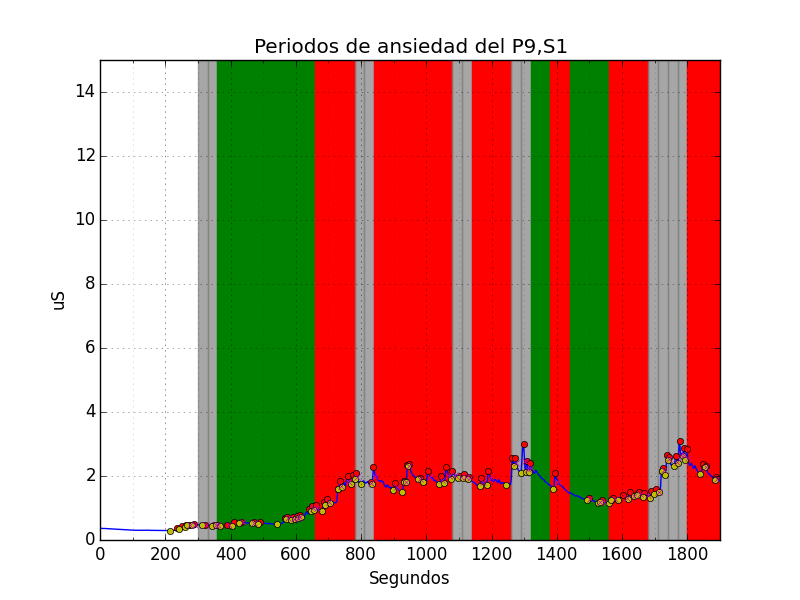
\includegraphics[height=80mm]{./Figures/img_SR_anxietyinduction.png}}
        \caption{Se\~nal de sudoraci\'on del participante 7. El periodo con fondo blanco incial corresponde al tiempo de relajaci\'on. Los periodos verdes corresponden a las etiquetas de no ansiedad y los rojos a los de ansiedad. Las secciones grises son segmentos ambiguos, en donde no se pudo determinar si hab\'ia o no ansiedad.}\label{fig:anxietyinduction}

\end{figure}

Unos segundos despu\'es, la PcD entra a la habitaci\'on y se presenta con el participante. En este periodo (entre el segundo 200 y el 300) se pueden obervar ligeros cambios en su nivel de sudoraci\'on. A partir del segundo 350 hasta el 650 la se\~nal crece ligeramente pero se mantiene dentro de un margen moderado. Esto puede ser debido a que durante ese periodo no recibi\'o est\'imulos muy fuertes, lo cual coincide con los segmentos que fueron reportados y catalogados como de no ansiedad. Cuando empiezan los periodos de ansiedad se registran aumentos s\'ubitos en la se\~nal como los que se observan alrededor del segundo 620 y 830. Si revisamos los datos de observaci\'on, tenemos eventos de comportamiento de la persona con demencia de nivel 2 al rededor del segundo 602. La porci\'on correspondiente del di\'alogo dice lo siguiente: \textit{``PcD: Oye.. ¿`usted sabe donde está mi mamá?''}\textit{``Participante: Ah.. no.''}\textit{``PcD: Yo me quiero ir con ella ya.''}. Esto da indicios de una relaci\'on entre los est\'imulos que utilizamos y la respuesta fisiol\'ogica.

Una de las diferencias sustanciales de este estudio es la forma en que el participante recibe los est\'imulos. En los experimentos de laboratorio, el participante se encuentra en un entorno aislado y controlado. Se establecen frecuencias e intensidades exactas para los est\'imulos. Esto resulta en se\~nales fisiol\'ogicas mas limpias y f\'aciles de interpretar. En este estudio, al tener una situaci\'on mas parecida a la realidad, se tiene obtiene claramente una se\~nal con mas ruido y mas dif\'icil de interpretar. Un ejemplo muy claro se observa en la se\~nal de sudoraci\'on. En un experimento de laboratorio, si vemos un segmento de datos el participante tiene un periodo de relajaci\'on, un est\'imulo de unos segundos y otro periodo inmediato de relajaci\'on se ver\'ia como en la figura ~\ref{fig:gsrsynth}. En este estudio, por el contrario, la se\~nal no vuelve a su nivel inicial (ver figura ~\ref{fig:gsrstudy}). %en coclusiones poner que se necesitan mas estudios con este tipo de datos para ver como se comportarian en situaciones naturalistas

\begin{figure}[h!]
        \centering
        \subfigure[]{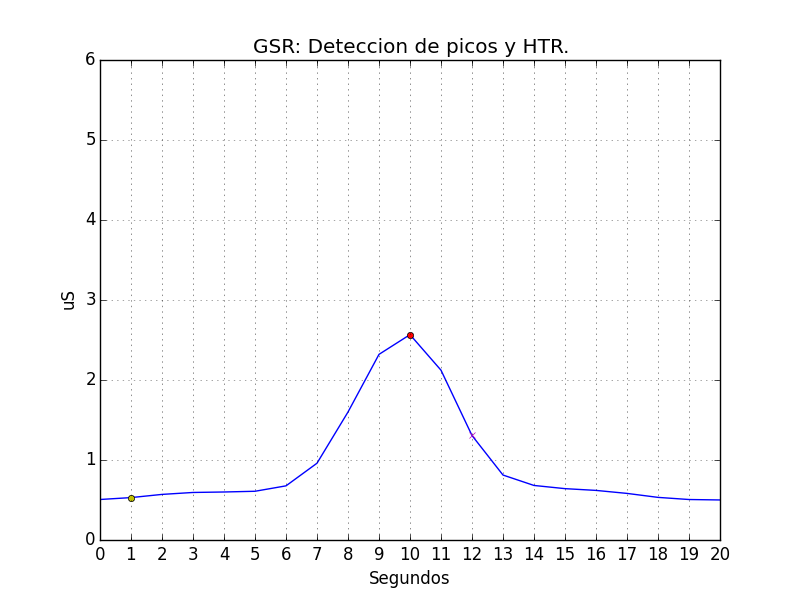
\includegraphics[height=70mm]{./Figures/img_synth.png}}
        \caption{Ejemplo de se\~nal de sudoraci\'on comunmente encontrado en otros estudios. Los periodos de relajaci\'on anteriores y posteriores al est\'imulo permiten identificar la respuesta fisiol\'ogica del participante.}\label{fig:gsrsynth}
\end{figure}
\begin{figure}[h!]
        \centering
        \subfigure[]{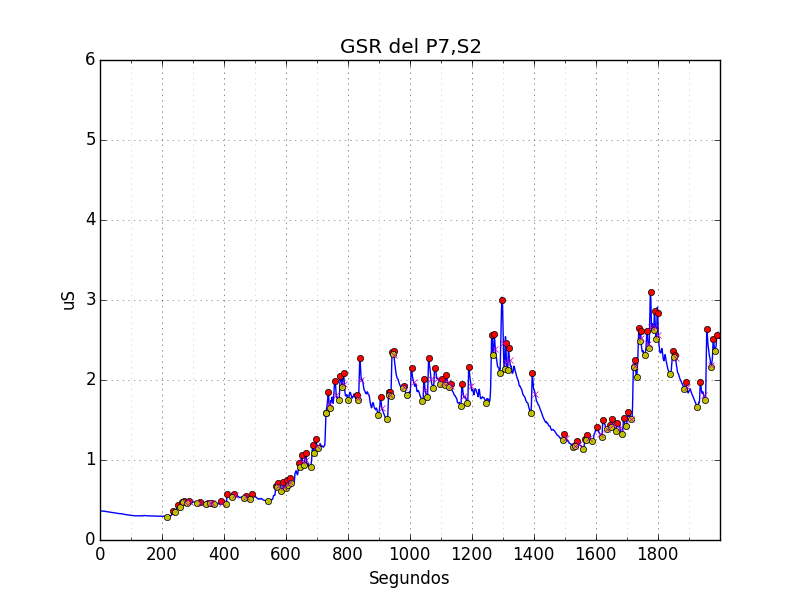
\includegraphics[height=70mm]{./Figures/img_p7s1.png}}
        \caption{Se\~nal de sudoraci\'on perteneciente al participante7, sesi\'on 1. La se\~nal no vuelve a su valor inicial antes del est\'imulo.}\label{fig:gsrstudy}
\end{figure}

Otra de las se\~nales relacionadas con la ansiedad y las emociones en general es el IBI \citep{Cinaz13}. Existe una relaci\'on entre la relajaci\'on y el IBI. Entre mas espaciados se encuntran los latidos del coraz\'on, podr\'ia indicar que la persona se encuentra m\'as relajado. Entre m\'as cortos sean, la persona se puede encontrar mas estresado. En este experimento se observ\'o un fen\'omeno muy directo sobre la se\~nal. Durante el periodo de relajaci\'on los valores de IBI tend\'ian a ser mas cercanos a 1.0, mientras que en los periodos de la prueba el valor tend\'ia a 0.4. En la figura ~\ref{fig:ibianxiety} se puede observar como durante los primeros 200 segundos (parte del periodo de relajaci\'on) los latidos son mas espaciados, mientras que durante la prueba y mas espec\'ifico a ciertas regiones el valor disminuye. Al rededor del segundo 700 se observa un valle mucho mas bajo que el resto de la se\~nal el cual puede estar relacionado con un evento de ansiedad. En general, la se\~nal de IBI se ve como una manifestaci\'on de un efecto fisiol\'ogico mas relacionado y sensible a los efectos de la ansiedad.

\begin{figure}[h!]
        \centering
        \subfigure[]{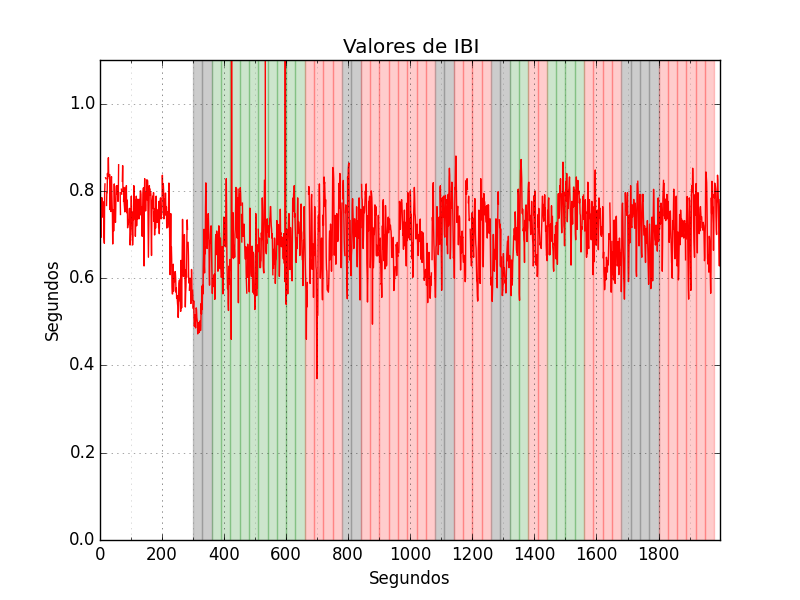
\includegraphics[height=80mm]{./Figures/img_p7s1IBI.png}}
        \caption{Se\~nal de IBI del participante 7, sesi\'on 1. Los valores son mas bajos durante la actividad que durante el periodo de relajaci\'on. Los colores de fondo fueron aclarados para facilitar la observaci\'on.}\label{fig:ibianxiety}
\end{figure}

%\section{Observaciones por participante}
%\textbf{ESCRIBE ALGO AQUI PLS}
%A continuaci\'on se muestran los datos de los participantes caso por caso

%\section{Datos crudos}


\section{Variaci\'on entre participantes}
Como resultado del estudio, se esperaban variaciones en las se\~nales fisiol\'ogicas entre los participantes. En la se\~nal de GSR, algunos individuos mostraban picos muy marcados seguidos de una corta recuperaci\'on y una serie de picos adicionales. Otros mostraron casi nulo incremento, lo cual podr\'ia indicar que la persona no sinti\'o ansiedad o bien, que no manifiesta el efecto de la ansiedad a trav\'es de la sudoraci\'on. Algunos participantes muestran un crecimiento exponencial, el cual podr\'ia indicar que la persona experimenta niveles de ansiedad cada vez mas elevados. Otra posibilidad es de que la pieza pl\'astica que utiliza el dispositivo para colocarse en la mu\~neca cause que el sudor se mantenga en la piel y se acumule durante la sesi\'on. Un usuario que produzca mucho sudor podr\'ia causar este efecto y podr\'ia dificultar la interpretaci\'on del nivel de ansiedad. Esto da indicios de que una aplicaci\'on consciente de la ansiedad debe de tomar en cuenta que diferentes usuarios pueden reaccionar de manera diferente a un estresor. La figura ~\ref{fig:gsrparticipants} ilustra estos fen\'omenos.


\begin{figure}[h!]
        \centering
        \subfigure[]{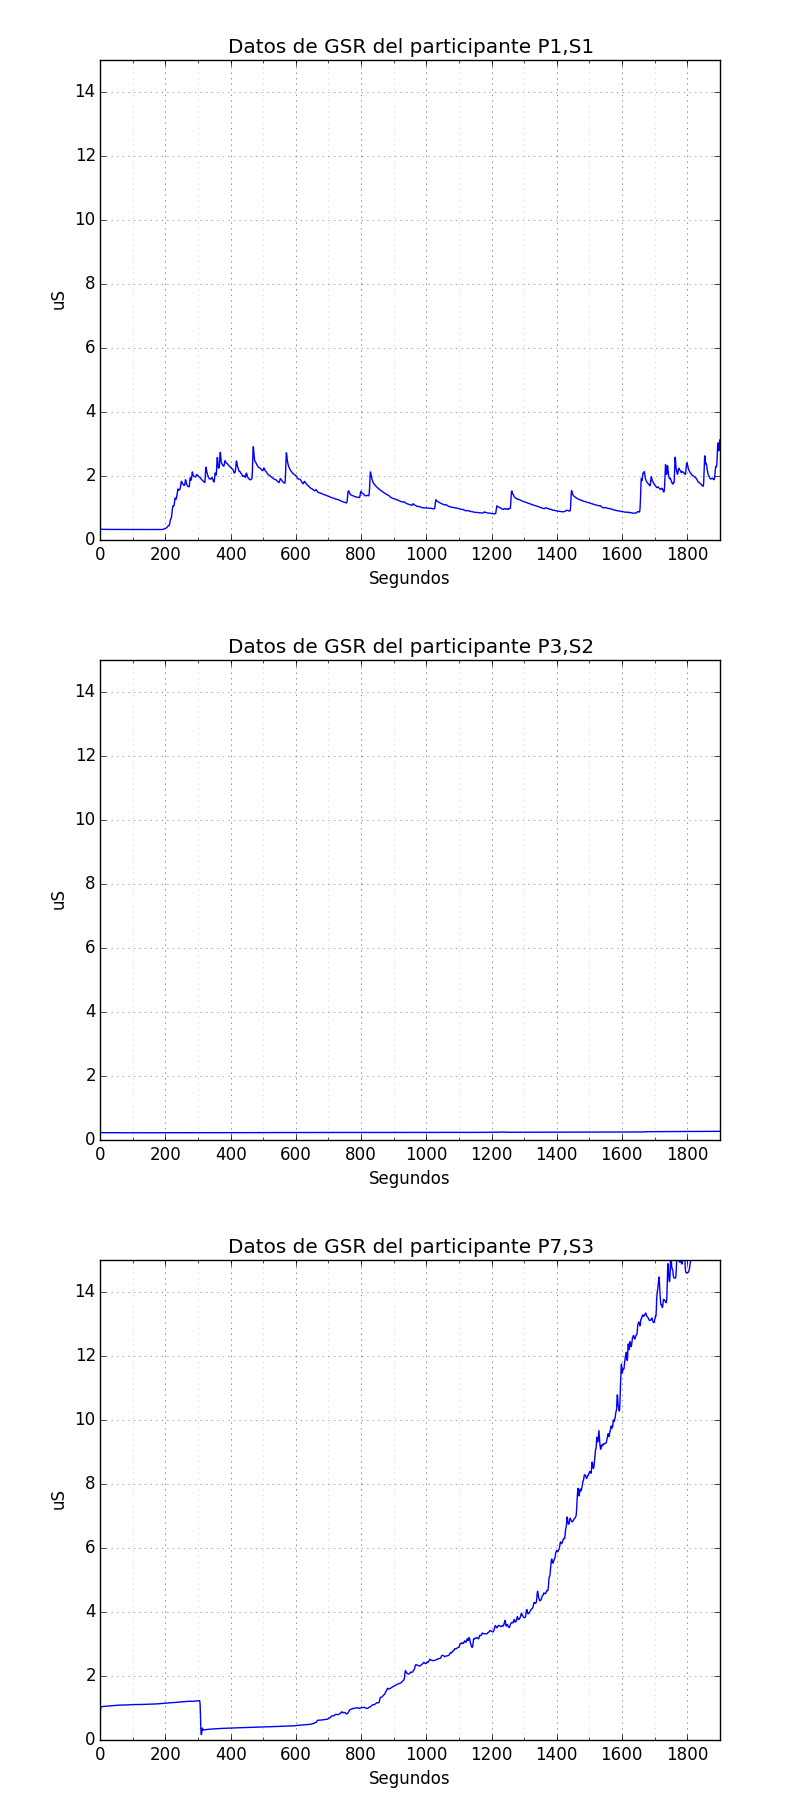
\includegraphics[height=160mm,width=220mm,keepaspectratio]{./Figures/img_gsrparticipants.png}}
        \caption{Se\~nal de GSR de tres diferentes participantes. Cada participante muestra una reacci\'on diferente a los est\'imulos de ansiedad.}\label{fig:gsrparticipants}
\end{figure}
Durante la fase de relajaci\'on, se observ\'o que el nivel de sudoraci\'on deca\'ia gradualmente hasta alcanzar un valor bajo de entre 0.1 y 1.0. Sin embargo, uno de los participantes en una sesi\'on en part\'icular se comport\'o de manera diferente. Su nivel inicial de sudoraci\'on fue muy alto, de al rededor de 14 \micro S, por lo que se tom\'o la decisi\'on de darle mas tiempo de relajaci\'on. Despu\'ues se reajust\'o el dispositivo para eliminar el sudor acumulado y se le pidi\'o que se volviera a relajar. El tiempo total de relajaci\'on fu\'e de 23:57 minutos. La figura ~\ref{fig:longrelax} ilustra este efecto. Una posible causa es que el participante se haya sentido ansioso mientras observaba al participante anterior realizar la terapia. Esta reacci\'on no se present\'o en las otras dos pruebas del mismo participante.


\begin{figure}[h!]
        \centering
        \subfigure[]{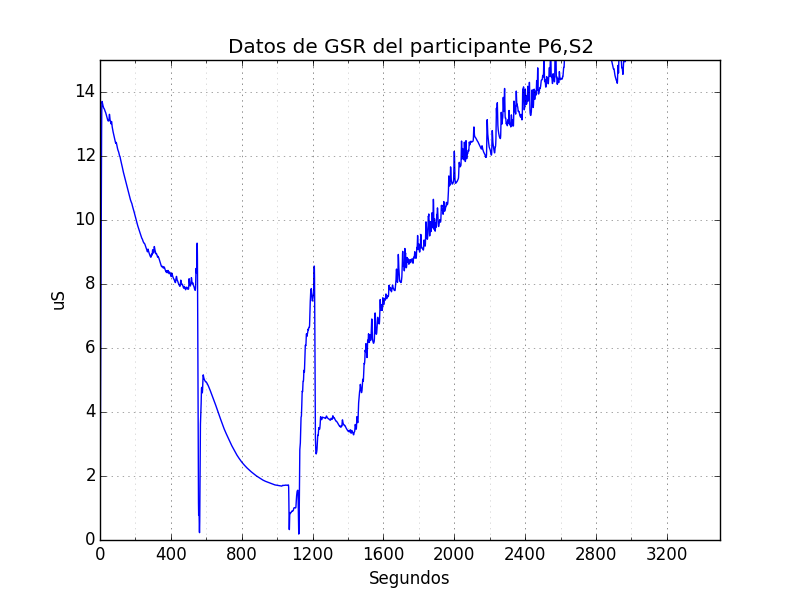
\includegraphics[width=130mm,keepaspectratio]{./Figures/img_longrelax}}
        \caption{Se\~nal de GSR del participante 6, sesi\'on 2. Se pueden observar m\'ultiples variaciones durante el periodo de relajaci\'on producto del estado emocional del participante y el ajuste del dispositivo. El pico s\'ubito del segundo 1100 corresponde al aviso de inicio de actividad.}\label{fig:longrelax}
\end{figure}


\section{Resultados de aprendizaje de m\'aquina}
La siguiente secci\'on muestra los resultados de las pruebas realizadas utilizando el algoritmo de clasif\'icaci\'on SVM. Todas las pruebas se hicieron utilizando la librer\'ia ``python-scikit''. Los datos de entrada fueron los vectores de caracter\'isticas obtenidos de los segmentos etiquetados como ``ansiedad'' y ``no ansiedad''. Los segmentos tuvieron una duraci\'on de 30 segundos. En todas las pruebas se utilizan 9 caracter\'isticas seleccionadas manualmente. Se realizaron diferentes pruebas con diferentes ``kernels'' de la m\'aquina de soporte vectorial. A continuaci\'on se muestran los resultados de cada una.

Se cont\'o con un total de 212 muestras de ansiedad y 310 de muestras de no ansiedad. (La tabla ~\ref{tab:anxietycounts} incluye a detalle los conteos de muestras)
\begin{table}[h!]
        \footnotesize
        \centering
        \caption{Conteos de muestras de ansiedad obtenidas}
\label{tab:anxietycounts}
%\rotatebox{90}{
        \begin{tabular}{m{.2cm}m{2.5cm}m{2.5cm}m{2.5cm}m{2.5cm}}
                \hline\noalign{\smallskip}
    &\textbf{Sujeto}&\textbf{Segmentos de ansiedad}&\textbf{Segmentos de no ansiedad}&\textbf{Segmentos ambiguos}\\
        \hline
 \\\noalign{\smallskip}
                &\textbf{P1}&36&28&42\\
                &\textbf{P6}&24&96&30\\
                &\textbf{P7}&70&68&16\\
                &\textbf{P8}&60&62&6\\
                &\textbf{P9}&22&56&22\\
                &\textbf{Total}&212&310&116
    \end{tabular}
\end{table}
\subsection{Pruebas por sujeto}
En aprendizaje de m\'aquina, precisi\'on es un resultado de relevancia, mientras que exhaustividad es una medidad de cuantos resultados relevantes est\'a regrsando. Un sistema con alta exhaustividad y baja precisi\'on regresa muchos resultados, pero la mayor\'ia de las etiquetas son incorrectas comparandolos con ``ground truth''. Un sistema con alta precisi\'on y baja exhaustividad es lo contrario, regresa muy pocos resultados pero la mayor\'ia de las etiquetas son correctas comparadas con ``ground truth''.

 La precisi\'on nos dice el porcentaje de muestras positivas clasificadas correctamente mas los falsos positivos mientras que la exhaustividad indica el porcentaje de muestras positivas clasificadas correctamente mas los falsos negativos. Por lo general, un sistema que utiliza aprendizaje de m\'aquina debe de tener valores altos de ambas medidas. Sin embargo, dependiendo de la aplicaci\'on, un valor alto de los dos es suficiente para realizar bien la tarea. A continuaci\'on se muestran diferentes pruebas y se utilizan la precisi\'on y exhaustividad para interpretar los resultados.

Un primer enfoque para la detecci\'on de ansiedad fue por medio del entrenamiento de un modelo personal. Este enfoque es utilizado debido a que las caracter\'isticas de las se\~nales fisiol\'ogicas pueden cambiar de individuo a individuo. Para esta prueba se utiliz\'o el 80\% de los datos de cada participante como entrenamiento y el 20\% restante para pruebas. En esta prueba se obtuvieron valores de precisi\'on y exhaustividad bajos.
Una posible raz\'on de este resultado es el hecho de que se cuenta con una baja cantidad de muestras de cada clase. La primera fila de la tabla ~\ref{table:resultindiv}, utilizando GSR e IBI para el P1 muestra estos valores.
\begin{table}[h!]
        \footnotesize
        \centering
        \caption{Resultados en la clasificaci\'on por participante.}
\label{table:resultindiv}
%\rotatebox{90}{
        \begin{tabular}{m{.2cm}m{1.5cm}m{1.5cm}m{1.5cm}m{1.5cm}m{1.5cm}m{1.5cm}m{1.5cm}m{2.5cm}}
                \hline\noalign{\smallskip}
    &\textbf{Sujeto}&\textbf{Se\~nal} &\textbf{Mtras. Entren.}&\textbf{Mtras. Prueba}&\textbf{Precisi\'on (Lin)}& \textbf{Recall (Lin)} & \textbf{Precis\'on (RBF)} &\textbf{Recall (RBF)}\\
	\hline                
 \\\noalign{\smallskip}
		&P1&GSR+IBI&22&6&60&50&42.86&50\\
		&P1&GSR&22&6&50&16.67&50&83.33\\
		&P1&IBI&22&6&50&50&60&50\\
		&P6&GSR+IBI&19&5&100&100&100&100\\
		&P6&GSR&19&5&100&20&66.67&40\\
		&P6&IBI&19&5&100&100&100&100\\
		&P7&GSR+IBI&54&14&48.15&92.86&30&21.43\\
		&P7&GSR&54&14&14.29&7.14&27.27&21.43\\
		&P7&IBI&54&14&48.15&92.86&33.33&7.14\\
		&P8&GSR+IBI&48&12&25&8.33&64.29&75\\
		&P8&GSR&48&12&25&8.33&57.14&33.33\\
		&P8&IBI&48&12&42.11&66.67&80&66.67\\
		&P9&GSR+IBI&17&5&100&40&60&60\\
		&P9&GSR&17&5&100&20&100&40\\
		&P9&IBI&17&5&0&0&100&100\\
    \end{tabular}
\end{table}

\subsection{Prueba en conjunto}
Se realiz\'o una segunda prueba con los datos, en esta ocasi\'on se tom\'o el 80\% de todas sesiones de todos los participantes como entrenamiento, y el 20\% restante como prueba. En esta ocasi\'on, se obtienen valores de precisi\'on parecidos entre las se\~nales, con un exhaustividad baja. Esto podr\'ia significar que la cantidad de muestras es uno de los factores que afectan el rendimiento del clasificador para este conjunto de datos. La tabla ~\ref{table:resultsall} muestra los resultados.

\begin{table}[h!]
        \footnotesize
        \centering
        \caption{Resultados en la clasificaci\'on en conjunto.}
\label{table:resultsall}
%\rotatebox{90}{
        \begin{tabular}{m{.2cm}m{3.0cm}m{1.5cm}m{1.5cm}m{1.5cm}m{1.5cm}m{1.5cm}m{1.5cm}m{1.5cm}}
                \hline\noalign{\smallskip}
    &\textbf{Sujeto}&\textbf{Se\~nal} &\textbf{Mtras. Entren.}&\textbf{Mtras. Prueba}&\textbf{Precisi\'on (Lin)}& \textbf{Recall (Lin)} & \textbf{Precis\'on (RBF)} &\textbf{Recall (RBF)}\\
	\hline                
 \\\noalign{\smallskip}
&P1+P6+P7+P8+P9&GSR+IBI&169&43&81.48&51.16&75&48.84\\
&P1+P6+P7+P8+P9&GSR&169&43&71.43&11.63&68.18&34.88\\
&P1+P6+P7+P8+P9&IBI&169&43&71.88&53.49&76.67&53.49\\


    \end{tabular}
\end{table}
\subsection{Pruebas entre sujetos}
La siguente prueba tom\'o en cuenta la necesidad de tener una mayor cantidad de datos y que al mismo tiempo fuera aplicable para la detecci\'on de ansiedad para un participante en espec\'ifico. Se tomaron los datos de las tres sesiones del participante a probar y todo el conjunto restante como entrenamiento. Esto se hizo para todos los participantes disponibles con las tres se\~nales. Se encontr\'o una precisi\'on alta en la mayor\'ia de los casos mientras que el ``recall'' permaneci\'o muy bajo utilizando un kernel lineal. En el caso del kernel RBF, los resultados fueron bajos. (Ver tabla: ~\ref{table:resultsCross}). Una variante de esta prueba, fue utilizar un kernel polinomial. En este caso, se obtuvo puntajes altos en precisi\'on y recall para la mayor\'ia de los casos.

\begin{table}[h!]
        \footnotesize
        \centering
        \caption{Resultados en la clasificaci\'on entre sujetos usando kernels lineales y RBF.}
\label{table:resultsCross}
%\rotatebox{90}{
        \begin{tabular}{m{.2cm}m{2.5cm}m{1.2cm}m{1.2cm}m{1.2cm}m{1.2cm}m{1.2cm}m{1.2cm}m{1.2cm}m{1.2cm}}
                \hline\noalign{\smallskip}
    &\textbf{Sujetos de entren.}&\textbf{Sujeto de prueba}&\textbf{Se\~nal} &\textbf{Mtras. Entren.}&\textbf{Mtras. Prueba}&\textbf{Precisi\'on (Lin)}& \textbf{Recall (Lin)} & \textbf{Precis\'on (RBF)} &\textbf{Recall (RBF)}\\
	\hline                
 \\\noalign{\smallskip}
			&P6+P7+P8+P9&P1&GSR+IBI&176&36&43.55&20.15&57.5&34.33\\
			&P6+P7+P8+P9&P1&GSR&176&36&33.33&1.49&68.97&14.93\\
			&P6+P7+P8+P9&P1&IBI&176&36&46.27&23.13&62.5&44.78\\
			&P1+P7+P8+P9&P6&GSR+IBI&188&24&66.67&13.11&86.21&40.98\\
			&P1+P7+P8+P9&P6&GSR&188&24&68&13.93&83.33&61.48\\
			&P1+P7+P8+P9&P6&IBI&188&24&76.47&42.62&92.54&50.82\\
			&P1+P6+P8+P9&P7&GSR+IBI&142&70&53.28&38.69&60.74&48.81\\
			&P1+P6+P8+P9&P7&GSR&142&70&47.06&14.29&57.5&27.38\\
			&P1+P6+P8+P9&P7&IBI&142&70&56.78&39.88&58.49&55.36\\
			&P1+P6+P7+P9&P8&GSR+IBI&152&60&100&4.43&92&29.11\\
			&P1+P6+P7+P9&P8&GSR&152&60&100&2.53&88&27.85\\
			&P1+P6+P7+P9&P8&IBI&152&60&69.02&80.38&100&38.61\\
			&P1+P6+P7+P8&P9&GSR+IBI&190&22&74.07&16.67&84.62&27.5\\
			&P1+P6+P7+P8&P9&GSR&190&22&100&8.33&86.11&25.83\\
			&P1+P6+P7+P8&P9&IBI&190&22&72.22&21.67&88.33&44.17\\

    \end{tabular}
\end{table}

\begin{table}[h!]
        \footnotesize
        \centering
        \caption{Resultados en la clasificaci\'on entre sujetos usando un kernel polinomial.}
\label{table:resultsCross}
%\rotatebox{90}{
        \begin{tabular}{m{.2cm}m{2.5cm}m{1.2cm}m{1.2cm}m{1.2cm}m{1.2cm}m{1.2cm}m{1.2cm}m{1.2cm}m{1.2cm}}
                \hline\noalign{\smallskip}
    &\textbf{Sujetos de entren.}&\textbf{Sujeto de prueba}&\textbf{Se\~nal} &\textbf{Mtras. Entren.}&\textbf{Mtras. Prueba}&\textbf{Precisi\'on (Poly)}& \textbf{Recall (Poly)}\\
	\hline                
 \\\noalign{\smallskip}
&P6+P7+P8+P9&P1&GSR+IBI&176&36&73.72&75.37\\
&P6+P7+P8+P9&P1&GSR&176&36&0&0\\
&P6+P7+P8+P9&P1&IBI&176&36&70&62.69\\
&P1+P7+P8+P9&P6&GSR+IBI&188&24&87.63&69.67\\
&P1+P7+P8+P9&P6&GSR&188&24&86.13&96.72\\
&P1+P7+P8+P9&P6&IBI&188&24&76.92&8.2\\
&P1+P6+P8+P9&P7&GSR+IBI&142&70&65.91&69.05\\
&P1+P6+P8+P9&P7&GSR&142&70&37.5&3.57\\
&P1+P6+P8+P9&P7&IBI&142&70&63.33&67.86\\
&P1+P6+P7+P9&P8&GSR+IBI&152&60&72&91.14\\
&P1+P6+P7+P9&P8&GSR&152&60&72.56&98.73\\
&P1+P6+P7+P9&P8&IBI&152&60&72.17&96.84\\
&P1+P6+P7+P8&P9&GSR+IBI&190&22&77.27&28.33\\
&P1+P6+P7+P8&P9&GSR&190&22&100&0.83\\
&P1+P6+P7+P8&P9&IBI&190&22&94.74&15\\
    \end{tabular}
\end{table}
\newpage
\subsection{Prueba por sesi\'on}
Por \'ultimo, se realiz\'o una prueba para comparar la informaci\'on de ``ground truth'' con el modelo general. La gr\'afica ~\ref{fig:gtvspredict} muestra dicha comparaci\'on. Se utiliz\'o un filtro de erosi\'on sobre los datos de predicci\'on para ajustar los periodos en donde el clasificador no detectaba ansiedad. Como resultado, muestra dos grandes bloques que indican periodos de ansiedad y uno peque\~no, en donde detecta ansiedad cuando no lo hay.

\begin{figure}[h!]
        \centering
        \subfigure[]{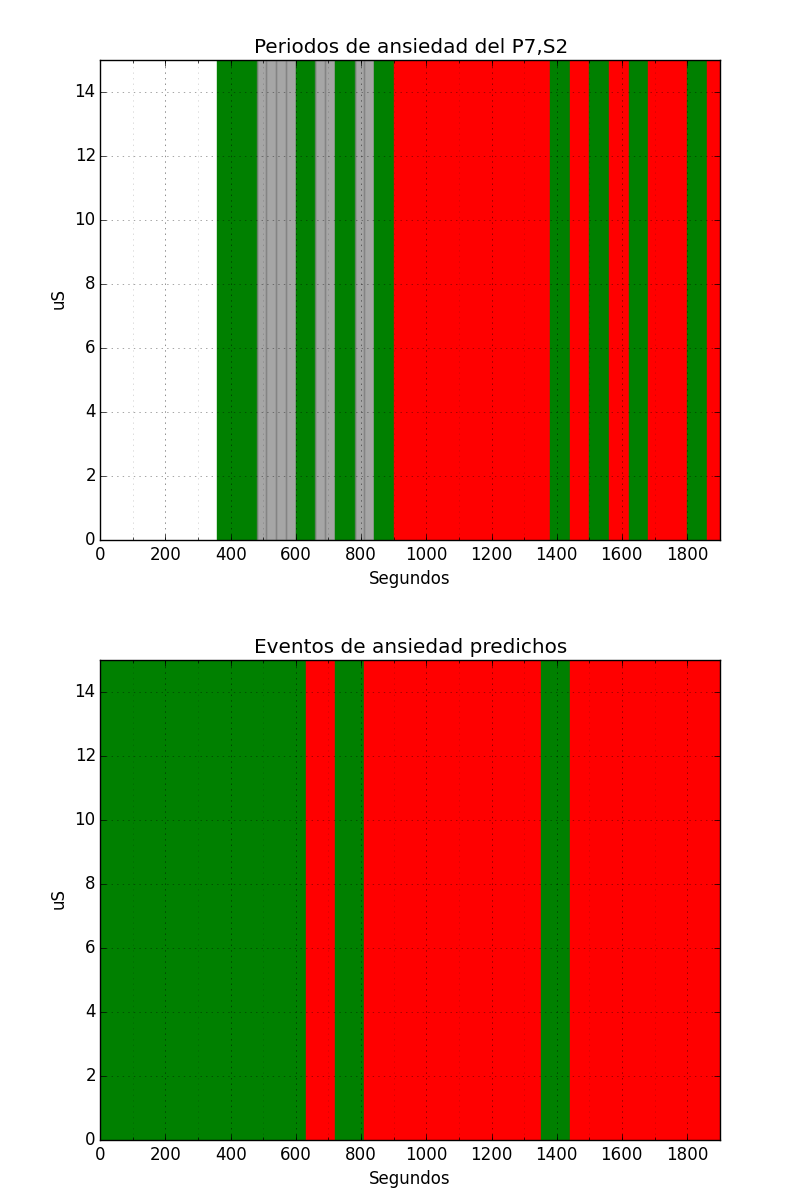
\includegraphics[height=130mm]{./Figures/img_prediction.png}}
        \caption{Comparaci\'on de los eventos de ansiedad predichos (gr\'afica inferior) por el modelo de SVM con ground truth (gr\'afica inferior).}\label{fig:gtvspredict}

\end{figure}

\section{Conclusi\'on}
	El dise\~no de este experimento muestra que es posible obtener datos fisiol\'ogicos de cuidadores en situaciones naturalistas. Se explor\'o como estas situaciones afectan a los datos obtenidos y se di\'o una primera aproximaci\'on a las t\'ecnicas necesarias para procesar datos en estas condiciones. Se mostr\'o tambi\'en que t\'ecnicas se pueden utilizar para solventar las deficiencias del m\'etodo y se muestra un conjunto de datos en el que se puede trabajar para desarrollar mejores t\'ecnicas de detecci\'on de ansiedad.
\newpage
%%=====================================================
